\documentclass[9.5 pt]{article}
\usepackage[letterpaper, portrait, margin = 1 in]{geometry}
\usepackage{amsmath}
\usepackage{amssymb}
\usepackage{amsfonts}
\usepackage{graphicx}
\graphicspath{{images/}}
\usepackage{nicefrac}
\usepackage{setspace}
\usepackage{bbm} 
\usepackage{hyperref}
\usepackage{pdfpages}
\usepackage{mathtools}
\usepackage{wrapfig}
\usepackage{chronosys,tabularx,langsci-optional}
\newcommand\tab[1][0.75cm]{\hspace*{#1}}
\setlength\parindent{0pt} %no indentation by default
\usepackage{parskip}
\setlength{\parindent}{15pt}
\usepackage{float} %for manual placement of floats (images, tables, etc.)
\hypersetup{
    colorlinks=true,
    allcolors=blue}
\usepackage{colortbl} %for coloring in cells of tables
\usepackage{dsfont} %for characteristic function (fancy 1)
\usepackage{subcaption}
\usepackage{subcaption}
\DeclareCaptionSubType*[Alph]{table}
\DeclareCaptionLabelFormat{mystyle}{Table~\bothIfFirst{#1}{ ̃}#2}
\captionsetup[subtable]{labelformat=mystyle}
\usepackage{enumitem}
\usepackage{amsmath}
\usepackage{setspace}
\onehalfspacing

\title{\textbf{STSCI 4740 Course Project}}
\date{Friday, December 7, 2018}
\author{Elva Lau (eml229), Lucus Tse (lyt6), Jamie Wong (jmw488), Joshua Ying(jmy48), \\ Christina Zhao (cfz8)}
\begin{document}
\pagenumbering{gobble}% Remove page numbers (and reset to 1)
\clearpage
\thispagestyle{empty}
\maketitle
\pagebreak
\pagenumbering{roman}
\tableofcontents %remove if preferred
\pagebreak


%********************************** 1 Introduction **********************************
\pagebreak[4]
\pagenumbering{arabic}
\setcounter{page}{1}

\section{Introduction}
Our team was tasked with using Machine Learning methods to uncover what variables are important towards predicting 23 distinct job categories at Google. That is, if someone were to apply to Google, we want to see what kind of job category he or she would fit the best in based on his or her qualifications, location, background, etc.  Our team was given a data set consisting of 1250 job descriptions with 7 features. Through data cleaning, manipulation, and feature engineering and then applying various machine learning methods, we were able to predict each job category with an 83.5\% accuracy from 5-fold cross validation.

%********************************** 3 PROBLEM Description & APPROACH **********************************
\section{Problem Approach and Data Transformation}
\subsection{Data Cleaning and Feature Engineering}
\par Our dataset consists of 1250 job descriptions from Google with seven features: Company, Title, Category, Location, Responsibilities, Minimum Qualifications, Preferred Qualifications. 
\subsubsection{Removing Unnecessary Features} 
There were a few features that we did not consider in our data set. Given that the objective we are trying to predict is an applicant's job category based on applicant characteristics, we removed the 'Title' feature. We removed 'Title' because the job title is not an attribute of a potential job applicant but is more of a redundant non-prediction feature that has a high interaction with Category. We believe that a potential applicant's job category cannot be predicted using the job title because they are so correlated that job title is essentially the response we are interested in. In the case that we do include job title, statistical learning wouldn't be necessary because Google's job titles are already bucketed into respective job categories. \\ \\
We also removed the 'Company' feature because it has a variance of 0, providing no predictive information.

\subsubsection{Combining Categories}
The 'Category' feature consisted of 23 categories that were incredibly imbalanced; i.e. the category counts ranged from 2 to 161. This would produce large prediction inaccuracies, especially for smaller categories. \par
We reduced the 'Category' feature from 23 to 7 categories roughly based on how Google classifies each Category on their careers website: \textbf{Business, Marketing, Engineering \& Design (ED), Sales, Internal Operations (IO), Developer Relations \& Technical Solutions (DRTS), and Operations and Support (OS)}. The new 7 categories that we use in our predictive model now range from a count of 102 to 247. This change drastically improved our test accuracy from around 30\% to around 80\% when comparing the data the models we tried using the pre-combined Categories and the post-combined Categories. 

\begin{figure}
\centering
\begin{subfigure}{.5\textwidth}
  \centering  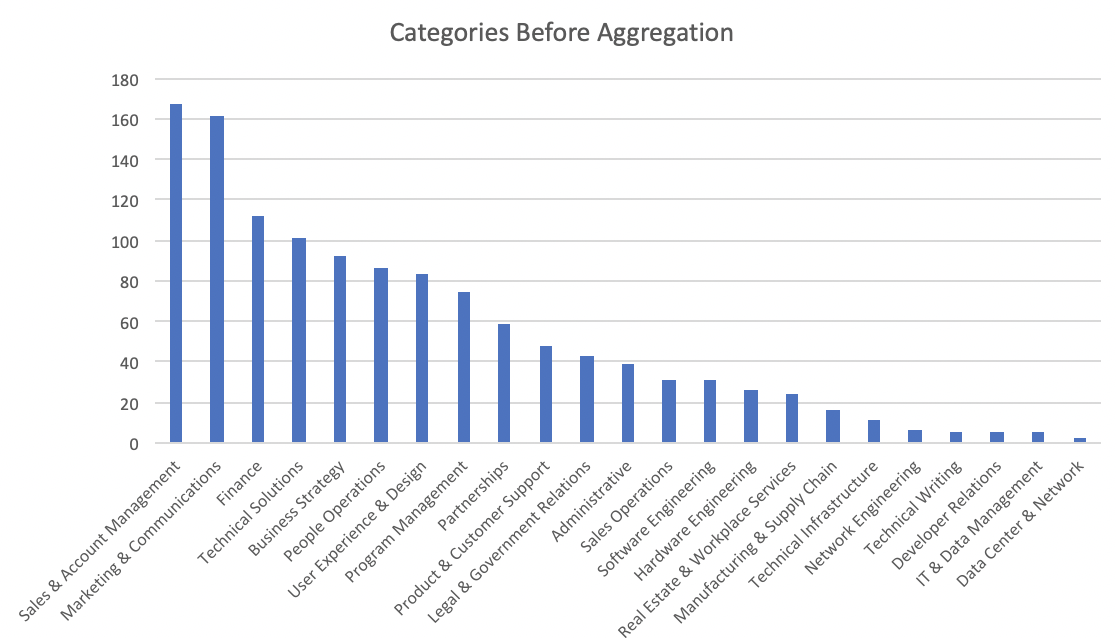
\includegraphics[width=1\linewidth]{Categories.png}
  \caption{'Category' before}
  \label{fig:sub1}
\end{subfigure}%
\begin{subfigure}{.5\textwidth}
  \centering
  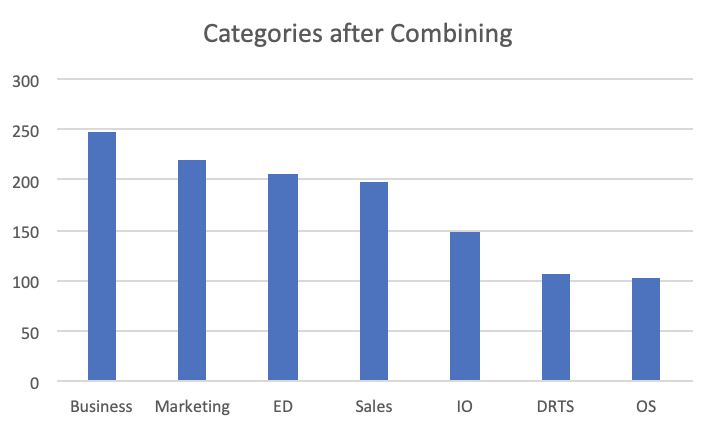
\includegraphics[width=1\linewidth]{categoriesafter.png}
  \caption{'Category' after}
  \label{fig:sub2}
\end{subfigure}
\caption{Combining 23 Categories into 7}
\label{fig:test}
\end{figure}
\vspace{1.5}
\subsubsection{Converting Categorical to Numeric}
Many of the models we tested required the categorical features to be numeric. To account for this, we used a dummy coding (one-hot-encoding) method to represent 'Category' and 'Location' features. i.e. (1,0,0,0) represents China and (0,1,0,0) represents USA. 

\subsubsection{Term Frequency Encoding}
The 'Responsibilities','Minimum Qualification', and 'Preferred Qualification' features consisted of long paragraphs describing ideal applicant attributes. To extract important words as features from these columns, we constructed feature-specific vocabularies of words and encoded these features as term frequencies. As intermediary preprocessing steps, we removed common English stop words such as "The, A, An..." and words that appeared in a majority of data points, like "Google." We also stemmed words to common prefixes, so that the appearance of tokens "Computation" and "Computer" would become two appearances of "Comput`". This would reduce necessary dimensions and sparsity while maintaining predictive power. \\ \\
For example, if the original feature was "Responsibilities": ["Computer Engineering," "Networking Engineer", "Neural Networks"], it would become ["Responsibilities\_Comput`": [1,0,0], "Responsibilities\_Engineer`": [1,1,0],
"Responsibilities\_Network`": [0,1,1]]
"Responsibilities\_Neural`": [0,0,1]]. Our bag-of-words dataset was formed by transforming the "Responsibilities," "Minimum Qualifications," and "Preferred Qualifications" features into this format.

The result was creating a 1227x1571 high-dimensional dataset. To manage a dataset with $p > n$, we used models with implicit feature selection, regularization, and wide kernelization.

\subsubsection{Further Feature Extraction}
While looking at the 'Minimum Qualification' and 'Preferred Qualification' column, we saw many repeated attributes such as education experience (BS/BA/MS/PhD/MBA), years of study, and field of study. We wanted to extract these as individual features, so we used regex (regular expressions) and the R grepl function to find each attribute in every column and represent them as dummy coded variables. For example, to create the Minimum Education Experience column, we made a vector 'min\_bs' to check if the string 'BS' existed in our original 'Minimum Education' column. If it did exist, we encoded that observation as 1 in the new 'min\_bs' column.
\begin{itemize}
    \item Extract Minimum Education Experience from Minimum Qualification
    \item Extract Preferred Education Experience from Preferred Qualifications
    \item Extract Years Required from Minimum Qualification
    \item Extract Field of study from Minimum Qualification
\end{itemize}

\subsection{Final Feature Engineered Dataset}
\begin{center}
   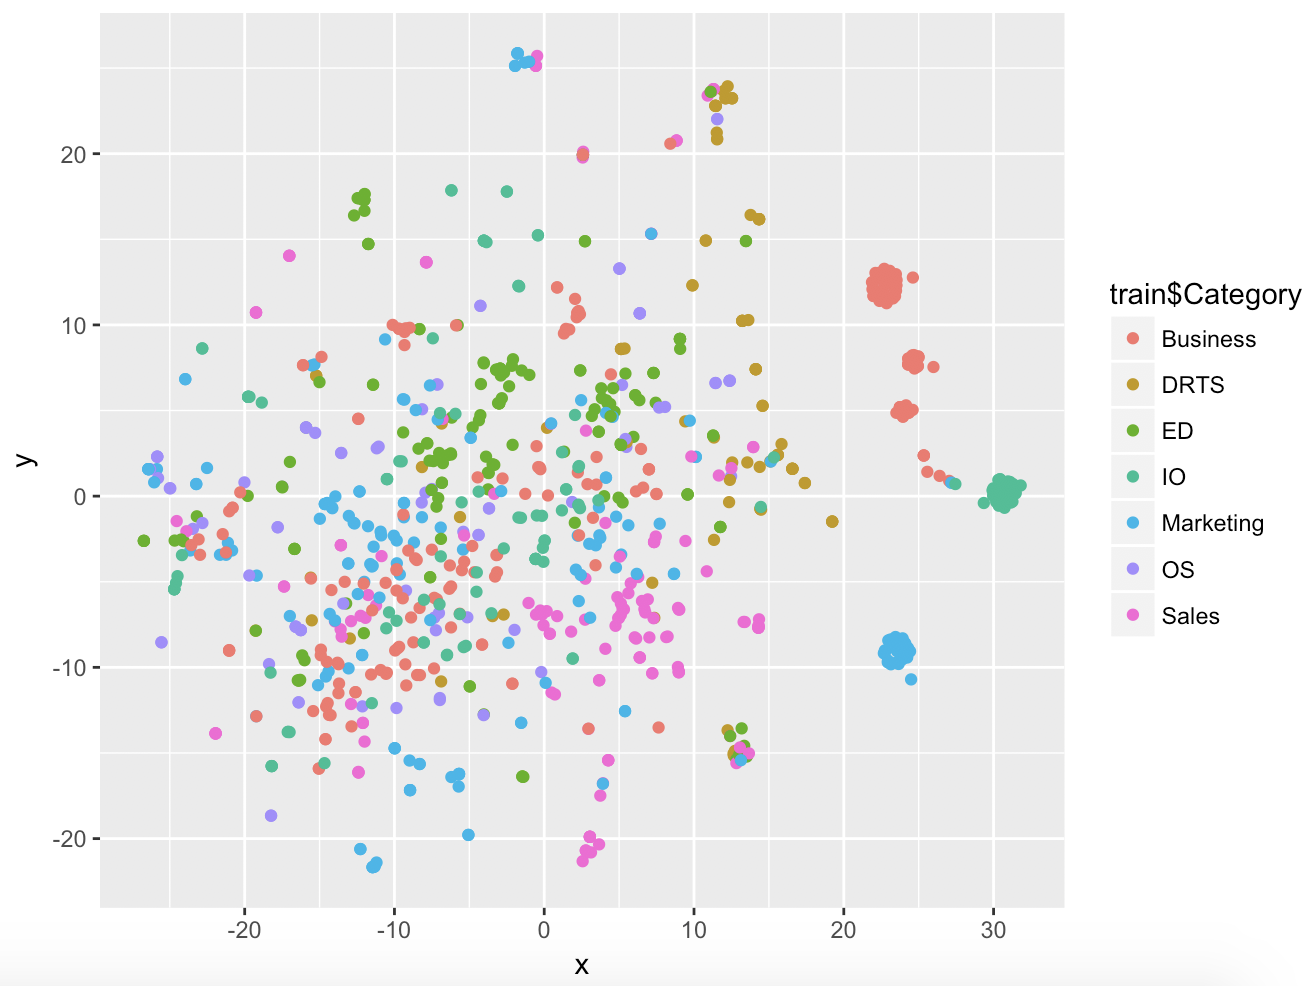
\includegraphics[width=1\textwidth]{tsne1.png}
 \end{center}
\caption{t-SNE visualization output}

Our final dataset consisted of 1388 features and 1227 observations. To demonstrate what our data looks like in 2D, we used t-SNE algorithm that uses the PCA algorithm to project high dimensional data onto 2D so that the high dimensional clustering is preserved. \par

From the 2D distance between data points in the t-SNE cluster visualization, we can understand the high dimensional distance in features of the data points. Immediately we can tell that 'Business', Engineering and Design ('ED'), as well as the 'Marketing'  categories have distinct clusters on the outer right along with larger clusters in the middle. On the other hand, the internal operations ('IO') category is more spread out; this may suggest that for this category, it is difficult to predict based on our extracted features whether an applicant belongs to the 'IO' category. 



\subsection{Train-Test Split Choice and \\ Reasoning}
We decided to use a 80\% of our data for our train set and 20\% of the data for our test set. In order to make up for a smaller test set, we performed parameter search using repeated 5-fold cross validation on the training set and compared individual models using the held out test set.


%********************************** 4 MODEL and Feature Selection **********************************
\section{Model Selection and Tuning}
\subsection{Stochastic Gradient Boosting}
As a starting point, due to the smaller size of the dataset, we wanted to aggregate regularization methods to combat overfitting. Boosting, or ensembling of weak learners, naturally regularizes. Introducing stochasticism, or bootstrapping the dataset for the individual learners, provided additional control over the variance of the model. Decision trees also naturally handle multiclass classification and different types of features.

The model was tuned using a 5-fold validated brute-force grid search on a parameter matrix of dimension 3x3x3. The stochastic gradient boosted model with a max-depth of 3, shrinkage value of 0.1, and 140 trees yielded an out-of-bag accuracy of .8378 and a kappa multiclass score of .8075. Resampling size and max leaf size were held constant at 980, 10 respectively.

\setlength{\arrayrulewidth}{1mm}
\setlength{\tabcolsep}{14pt}
\renewcommand{\arraystretch}{1.5}
 
\newcolumntype{s}{>{\columncolor[HTML]{898888}} p{1cm}}
 
\arrayrulecolor[HTML]{898888}

\begin{tabular}{||c c c c c c c c||} 
\hline
\rowcolor{orange} \multicolumn{8}{|l|}{Percentage Confusion Matrix: Stochastic Gradient Boosting} \\
\hline
\rowcolor{gray}
\cellcolor[HTML]{AA0044} Pred/True & Business & DRTS & ED & IO & Marketing & OS & Sales \\
\hline
\cellcolor{gray}  Business & 17.4 & 0.0 & 0.2 & 0.9 & 1.0 & 0.7 & 0.5 \\ \hline 
\cellcolor{gray}DRTS & 0.1 & 6.8 & 0.3 & 0.2 & 0.1 & 0.2 & 0.2 \\ \hline 
\cellcolor{gray}ED & 0.4 & 0.8 & 14.7 & 0.3 & 0.6 & 1.0 & 0.2 \\ \hline 
\cellcolor{gray}IO & 0.3 & 0.0 & 0.1 & 10.2 & 0.1 & 0.2 & 0.0 \\ \hline 
\cellcolor{gray}Marketing & 1.4 & 0.1 & 0.2 & 0.4 & 14.9 & 0.3 & 1.2 \\ \hline 
\cellcolor{gray}OS & 0.1 & 0.2 & 0.5 & 0.2 & 0.2 & 5.7 & 0.1 \\ \hline 
\cellcolor{gray}Sales & 0.5 & 0.7 & 0.7 & 0.0 & 1.1 & 0.2 & 13.9 \\
\hline
\end{tabular}

\subsection{L2 Regularized Multinomial Logistic Regression}
As with most classification problems, modeling probabilities for class membership and classifying the maximum probability class is a natural approach. We used a natural extension of the logistic model-- Multinomial Logistic Regression for unordered, multiple response categories to accommodate our data. Linear decision boundary loss based classifiers such as Logistic Regression also in theory address high dimensional space and the Curse of Dimensionality.

Logistic Regression routinely overfits data, especially high dimensional data, so we chose to test different kinds of regularization as an additional parameter.

\begin{minipage}[t]{0.6667\textwidth}
\setlength{\arrayrulewidth}{1mm}
\setlength{\tabcolsep}{12pt}
\renewcommand{\arraystretch}{1}
 
\newcolumntype{s}{>{\columncolor[HTML]{orange}} p{1cm}}
 
\arrayrulecolor[HTML]{898888}

\begin{tabular}{||c c c c c||} 
\hline
\rowcolor{orange} \multicolumn{5}{|c|}{Parameter Grid: Logistic Regression} \\
\hline
\rowcolor{gray}
Cost & Loss & Epsilon & Accuracy & Kappa \\ \hline
0.500 & L1 & 0.001 & 0.797 & 0.758 \\ \hline
0.500 & L1 & 0.010 & 0.800 & 0.762 \\ \hline
0.500 & L1 & 0.100 & 0.800 & 0.762 \\ \hline
0.500 & L2\_dual & 0.001 & 0.831 & 0.800 \\ \hline
0.500 & L2\_dual & 0.010 & 0.831 & 0.800 \\ \hline
0.500 & L2\_dual & 0.100 & 0.832 & 0.801 \\ \hline
0.500 & L2\_primal & 0.001 & 0.830 & 0.798 \\ \hline
0.500 & L2\_primal & 0.010 & 0.834 & 0.803 \\ \hline
0.500 & L2\_primal & 0.100 & 0.827 & 0.795 \\ \hline
1.000 & L1 & 0.001 & 0.805 & 0.768 \\ \hline
1.000 & L1 & 0.010 & 0.814 & 0.779 \\ \hline
1.000 & L1 & 0.100 & 0.812 & 0.777 \\ \hline
1.000 & L2\_dual & 0.001 & 0.829 & 0.797 \\ \hline
1.000 & L2\_dual & 0.010 & 0.829 & 0.797 \\ \hline
1.000 & L2\_dual & 0.100 & 0.829 & 0.797 \\ \hline
1.000 & L2\_primal & 0.001 & 0.829 & 0.797 \\ \hline
1.000 & L2\_primal & 0.010 & 0.829 & 0.797 \\ \hline
1.000 & L2\_primal & 0.100 & 0.832 & 0.801 \\
\hline
\end{tabular}
\end{minipage}
\begin{minipage}[t]{0.3333\textwidth}
\hfill
\parbox{1.0\textwidth}{
We see that the data favors a higher regularization cost with L1 and a lower cost for L2 during training. In general, L2 outperforms L1, suggesting a more uniform distribution of feature importance when compared to the sparse L1 models. This might point toward the fact that the presence of phrases, sentences, or combinations of tokens contributes more to the predictive power of the model rather than the presence of individual tokens, as the majority of the features are the feature-independent vocabularies. \\ \\
The highest accuracy is .834, achieved by L2 primal loss with convergence threshold of 0.01.
}
\end{minipage}

\subsection{Partial Least Squares with Wide Kernel}
In our third attempt to approach the high dimensional multi-classification problem, we wanted to try a regression algorithm and explore dimensional analysis, to cover distinct "families" of algorithms (ensembling/tree, classification, regression) to compare each technique's performance. For regression we chose Partial Least Squares, as it supposedly works well on high dimensional data due to its explicit multi-dimensional projection search. The algorithm automatically selects out multicollinear variables as well (by finding hyperplanes that encapsulate correlated data), of which we know there are many in our bag-of-words dataset. \\ \\
Additionally, we used an R implementation of the Wide Kernel algorithm for PLS, as it converged 2x faster on our high dimensional dataset.

\setlength{\arrayrulewidth}{1mm}
\setlength{\tabcolsep}{8pt}
\renewcommand{\arraystretch}{1.0}
 
\newcolumntype{s}{>{\columncolor[HTML]{898888}} p{1cm}}
 
\arrayrulecolor[HTML]{898888}

\begin{tabular}{||c c c c c c c c||} 
\hline
\rowcolor{orange} \multicolumn{8}{|l|}{PLS Feature Selection} \\
\hline
\rowcolor{gray}
\cellcolor[HTML]{266AFF} & Business & DRTS & ED & IO & Marketing & OS & Sales \\ \hline
\cellcolor[HTML]{266AFF} `Responsibilities\_partner` & 51.510 & 32.561 & 52.040 & 100.000 & 77.680 & 22.220 & 60.250 \\ \hline
\cellcolor[HTML]{266AFF} `Preferred.Qualifications\_design` & 28.550 & 13.711 & 79.740 & 30.320 & 35.870 & 32.220 & 49.490 \\ \hline
\cellcolor[HTML]{266AFF} `Responsibilities\_busi` & 31.840 & 19.623 & 79.600 & 42.900 & 23.970 & 36.140 & 69.250 \\ \hline
\cellcolor[HTML]{266AFF} `Responsibilities\_design` & 24.260 & 13.854 & 75.110 & 27.320 & 31.620 & 23.030 & 42.420 \\ \hline
\cellcolor[HTML]{266AFF} min\_years\_exp & 68.250 & 28.028 & 27.510 & 23.130 & 45.030 & 32.590 & 25.380 \\ \hline
\cellcolor[HTML]{266AFF} `Preferred.Qualifications\_abil` & 24.070 & 22.168 & 62.890 & 67.700 & 46.330 & 25.780 & 60.780 \\ \hline
\cellcolor[HTML]{266AFF} 
`Responsibilities\_client` & 34.880 & 25.944 & 50.610 & 67.650 & 46.890 & 34.390 & 51.700 \\ \hline
\cellcolor[HTML]{266AFF} 
`Responsibilities\_custom` & 50.500 & 43.198 & 67.460 & 65.360 & 27.680 & 25.110 & 63.770 \\ \hline
\cellcolor[HTML]{266AFF} 
`Responsibilities\_market` & 34.340 & 12.770 & 41.150 & 43.130 & 56.250 & 10.730 & 24.510 \\ \hline
\cellcolor[HTML]{266AFF} 
`Responsibilities\_product` & 36.430 & 31.060 & 53.250 & 44.430 & 50.230 & 19.580 & 32.480 \\ \hline
\cellcolor[HTML]{266AFF} 
`Preferred.Qualifications\_manag` & 20.150 & 20.700 & 23.490 & 52.950 & 29.450 & 32.730 & 25.640\\
\hline
\end{tabular}
\\\\Above are the most important features for the PLS model. Some interesting observations: the Responsibilities feature contains the most important variables. As we expected, the existence of category-specific terms greatly predicts category. "Partner" predicts IO, "design" predicts ED, business predicts Business, ED, Sales. Feature selection will be further discussed in the upcoming sections. \\ \\
The optimal PLS model was 30 components, producing an accuracy score of .8272.


%********************************** 5 MODEL EVALUATION **********************************
\section{Model Evaluation }

\subsection{Error Comparison}

For all models, the confusion matrices greatly resemble each other. (For reference, see the Stochastic Gradient Boosted confusion matrix). The values are generally very similar in magnitude. This, in combination with the fact that the 0-1 accuracies are very similar despite the relatively unique methods used point toward the fact that the data has a "hard limit" to generalization. There are not enough interactions and information encoded by the data that can discriminate particular problem points and similar category clusters, at least with the way we have set up bag-of-word encoding. \\ \\
A particular category interaction that is inherently difficult to differentiate is Marketing and Business. In all 3 confusion matrices there are .7-1.4\% of all data points classified as Marketing when true label is Business, and .7-1.1\% vice versa. Category pairs easy to discriminate are (IO, OS), (Marketing, DRTS), and (Sales, IO). This finding can be reproduced by language modeling words in vector spaces-- the words in Business and Marketing job descriptions are closer together in semantic vector space than Marketing and DRTS words. \\ \\
Note that the variance of standardized misclassified points of all categories for the Stochastic Gradient Boosted method is 0.1304, while the same metric is 0.0885 for Logistic Regression. This might be a consequence of the difference between how Tree ensembling and logistic modeling assigns predictions; decision trees will assign predictions to discrete leaves, which might produce more sparse predicted categories (especially with the nearsightedness of short trees) when compared to the continuous probabilistic modeling in the Logistic Regression algorithm. For this reason, and in conjunction with the slight accuracy increase, the L2 regularized Logistic Regression model is our model of choice.

\subsection{Feature Selection}

To explore feature selection even further, we performed One vs. All binary classification and examined the weights output by optimal models per category. We used 3-Fold Cross Validated, Class-weighted SVMs with L1-regularization for feature selection. The accuracy percentage averaged over all 7 categories ended up being 0.9094, although we take this with a grain of salt due to the possible large presence of type II errors. (when classifying category A with 100 observations vs. category B with 900, a trivial classifier that always classifies B will achieve .9 accuracy.)

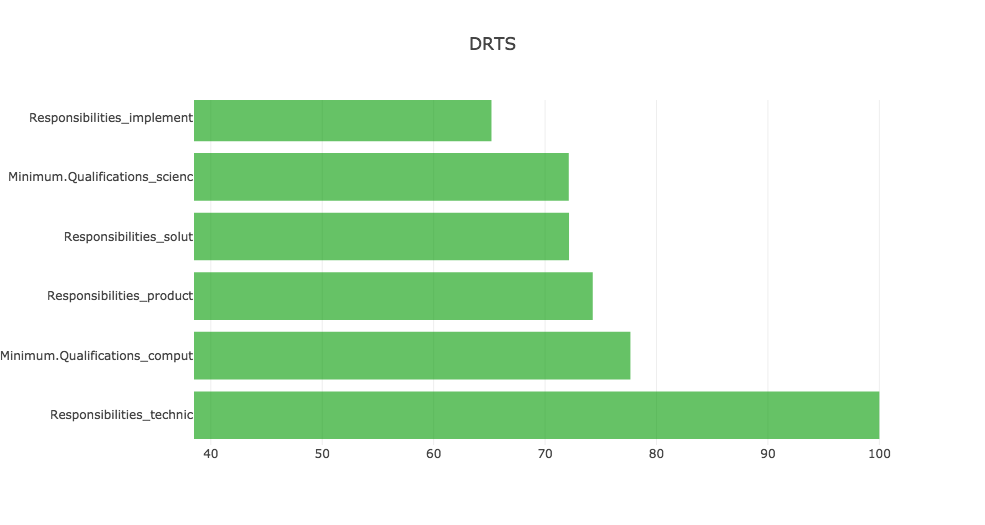
\includegraphics[scale=.35, trim=6cm 0 0 0cm]{newplot}
\includegraphics[scale=.35, trim=9cm 0 0 0cm]{"newplot (1)"}
\includegraphics[scale=.35, trim=4.5cm 0 0 0cm]{"newplot (2)"}
\includegraphics[scale=.35, trim=8cm 0 0 0cm]{"newplot (3)"}
\includegraphics[scale=.35, trim=4.5cm 0 0 0cm]{"newplot (4)"}
\includegraphics[scale=.35, trim=8cm 0 0 0cm]{"newplot (5)"}
\includegraphics[scale=.35, trim=5cm 0 0 0cm]{"newplot (6)"}


%********************************** 6 Conclusion **********************************

\section{Conclusion }
To summarize our findings-- our optimal model was L2 regularized Multinomial Logistic Regression, achieving 83\% classification accuracy on 7 categories. We found that aggressive regularization, randomization, bootstrapping, and kernel techniques were effective tools for handling high dimensional data. Somewhat unsurprisingly, the features that correlate with a particular job category include tokens in the actual job category: "Market" for Marketing, "Business" for Business, and so forth. Location provides little to no context for predicting job category. \\ \\
If we were to extend this project, we would explore word embeddings and vectorizations of the paragraphs in the Responsibilities, Minimum/Preferred Qualifications features. We would also explore LSTM networks, n-grams, and other canonical NLP techniques.
\end{document}